%%%%%%%%%%%%%%%%%%%%%%%%%
\section{\label{sec:lhs_nvt_bias}Biased canonical ensemble ($NVT$) trials}
%%%%%%%%%%%%%%%%%%%%%%%%%

In this section, biased $NVT$ trials are derived.
First, we consider AVB displacement trials.
Displacement trials include both linear and angular displacement.
There are a few variants of AVB to consider.
Although inefficiencies were found in the original version \cite{chen_aggregation-volume-bias_2001, wierzchowski_general-purpose_2001, wierzchowski_ub_2002}, the second variant, AVBMC2, efficiently moves particles in and out of the AV \cite{chen_improving_2001}.
A third variant, AVBMC3, allows for particles to move from the AV of one particle into the AV of another particle (denoted as ``in $\rightarrow$ in") \cite{chen_improving_2001}.
First, we introduce AVBMC2.
Then, we derive the ``in $\rightarrow$ in" part of AVBMC3, and then introduce a relatively new variant of AVBMC3 that we call AVBMC4 \cite{siderius_flat-histogram_2024}, which is very similar to AVBMC3 but allows for overlapping AVs.
After AVB, we also derive CB and DCCB displacements in the $NVT$ ensemble.

%%%%%%%%%%%%%%%%%%%%%%%%%
\subsection{\label{sec:lhs_disp_avb2}Displacement with aggregation volume bias (AVBMC2)}
%%%%%%%%%%%%%%%%%%%%%%%%%

\begin{figure}
\begin{centering}
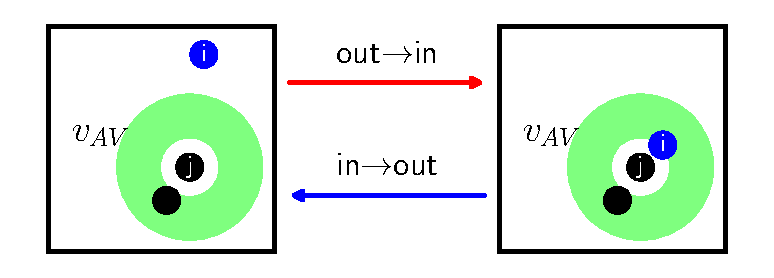
\includegraphics[width=6.5cm]{../figures/avb2.pdf}
\caption{
AVBMC2 displacement of a blue particle of type $i$ from outside to inside the AV, $v_{AV}$ shown in green, of an existing target particle of type $j$, and the reverse trial.
}
\label{fig:avbmc2}
\end{centering}
\end{figure}

In AVBMC2, a target particle of type $j$ is chosen randomly from $N_j$ particles.
The AV is then defined about one specific site in the target particle.
The mobile particle with one specific site then attempts a move into or out of the AV, with $N_i$ particles of this type.
The target and mobile particles may be the same.
In this case, $\delta_{ij}=1$, otherwise, $\delta_{ij}=0$.
At the beginning of the trial, there are $N_i^{AV}$ particles of type $i$ inside the AV of the specific site in the chosen particle of type $j$.
AVBMC2 is an $NVT$ trial because the total number of particles does not change.

In the AVB algorithm, it is possible for a particle to be inserted into an AV such that it happens to fall in the AV of two other particles, so that there would be more than one way to transition to the same microstate.
The transition probabilities do not need to account for this circumstance, because super-detailed balance is satisfied for each path.
The unbonding bonding (UB) algorithm \cite{wierzchowski_general-purpose_2001} presents a variation of the AVB algorithm that more explicitly accounts for these cases.

The AVBMC2 trial proceeds as follows.
A target particle of type $j$ is chosen randomly from $N_j$ and the AV is defined about the specific site in the chosen particle.
With probability $P_{bias}$, an ``out $\rightarrow$ in" trial is performed.
Otherwise, an ``in $\rightarrow$ out" trial is performed.
For ``out $\rightarrow$ in," one of $N_i$ particles of type $i$ is chosen randomly that has the specific site in $i$ that is not in the AV.
The chosen mobile site of the particle of type $i$ is then placed at a random position selected uniformly in the AV.
If the particle has other sites, they may then be regrown with CB or randomly rotated.
For ``in $\rightarrow$ out," one of the $N_i^{AV}$ sites in the AV is placed randomly in the entire simulation domain that is not in the AV.
Again, the remainder of the particle may then be oriented randomly or regrown with CB.

The transition probabilities for AVBMC2 are summarized in Table~\ref{tab:lhs_disp_in_avb2} for a forward transition of ``out $\rightarrow$ in."
The reverse move always has $N_i^{AV}+1$ in the AV, where $N_i^{AV}$ is the number of mobile sites in particles of type $m$ in the AV at the beginning of the trial.

\begin{table}
\begin{center}
\begin{tabular}{|c|c|}
 \hline
 \thead{Forward} & \thead{$\alpha_{o\rightarrow n}$} \\ [0.5ex]
 \hline
 Choose particle of type $j$ & $1/N_j$ \\
 \hline
 Choose ``out $\rightarrow$ in" & $P_{bias}$ \\
 \hline
 Choose mobile site not in AV & $1/(N_i - N_i^{AV} - \delta_{ij})$ \\
 \hline
 Choose $\mathbf{r}_n$ in AV & $\diff\mathbf{r}/v_{AV}$ \\
 \hline
 Choose orientation & $P_{\omega n}\diff\boldsymbol{\omega}$ \\
 \hline\hline
 \thead{Reverse} & \thead{$\alpha_{n\rightarrow o}$} \\ [0.5ex]
 \hline
 Choose particle of type $j$ & $1/N_j$ \\
 \hline
 Choose ``in $\rightarrow$ out" & $1-P_{bias}$ \\
 \hline
 Choose mobile site in AV & $1/(N_i^{AV} + 1)$ \\
 \hline
 Choose $\mathbf{r}_o$ outside AV & $\diff\mathbf{r}/(V - v_{AV})$ \\
 \hline
 Choose orientation & $P_{\omega o}\diff\boldsymbol{\omega}$ \\
 \hline
\end{tabular}
\caption{Particle displacement AVBMC2 ``out $\rightarrow$ in" transition probabilities.}
\label{tab:lhs_disp_in_avb2}
\end{center}
\end{table}

Using Table~\ref{tab:lhs_disp_in_avb2} and substituting Eq.~\ref{eq:rhs_nvt} into Eq.~\ref{eq:detailed_balance}, the acceptance probability is
\begin{equation}
\chi = \frac{P_{\omega o}(1-P_{bias})(N_i-N_i^{AV}-\delta_{ij})v_{AV}}{P_{\omega n} P_{bias}(N_i^{AV}+1)(V-v_{AV})}e^{-\beta \Delta U}.
\label{eq:avb2outin}
\end{equation}
For an example of combining AVB with CB, see the Appendix of Ref.~\cite{hatch_self-assembly_2016}.

The transition probabilities for ``in $\rightarrow$ out" as the forward transition are summarized in Table~\ref{tab:lhs_disp_out_avb2}.
Using Table~\ref{tab:lhs_disp_out_avb2} and substituting Eq.~\ref{eq:rhs_nvt} into Eq.~\ref{eq:detailed_balance}, the acceptance probability is
\begin{equation}
\chi = \frac{P_{\omega o} P_{bias}N_i^{AV}(V/v_{AV}-1)e^{-\beta \Delta U}}{P_{\omega n}(1-P_{bias})(N_i-N_i^{AV}-\delta_{ij}+1)}.
\label{eq:avb2inout}
\end{equation}

\begin{table}
\begin{center}
\begin{tabular}{|c|c|}
 \hline
 \thead{Forward} & \thead{$\alpha_{o\rightarrow n}$} \\ [0.5ex]
 \hline
 Choose particle of type $j$ & $1/N_j$ \\
 \hline
 Choose ``in $\rightarrow$ out" & $1-P_{bias}$ \\
 \hline
 Choose mobile site in AV & $1/N_i^{AV}$ \\
 \hline
 Choose $\mathbf{r}_n$ outside AV & $\diff\mathbf{r}/(V - v_{AV})$ \\
 \hline
 Choose orientation & $P_{\omega n}\diff\boldsymbol{\omega}$ \\
 \hline\hline
 \thead{Reverse} & \thead{$\alpha_{n\rightarrow o}$} \\ [0.5ex]
 \hline
 Choose particle of type $j$ & $1/N_j$ \\
 \hline
 Choose ``out $\rightarrow$ in" & $P_{bias}$ \\
 \hline
 Choose mobile site not in AV & $1/(N_i - N_i^{AV} - \delta_{ij} + 1)$ \\
 \hline
 Choose $\mathbf{r}_o$ in AV & $\diff\mathbf{r}/v_{AV}$ \\
 \hline
 Choose orientation & $P_{\omega o}\diff\boldsymbol{\omega}$ \\
 \hline
\end{tabular}
\caption{Particle displacement AVBMC2 ``in $\rightarrow$ out" transition probabilities.}
\label{tab:lhs_disp_out_avb2}
\end{center}
\end{table}

%%%%%%%%%%%%%%%%%%%%%%%%%
\subsection{\label{sec:lhs_disp_avb34}Displacement from one aggregation volume to another (AVBMC3/4)}
%%%%%%%%%%%%%%%%%%%%%%%%%

\begin{figure}
\begin{centering}
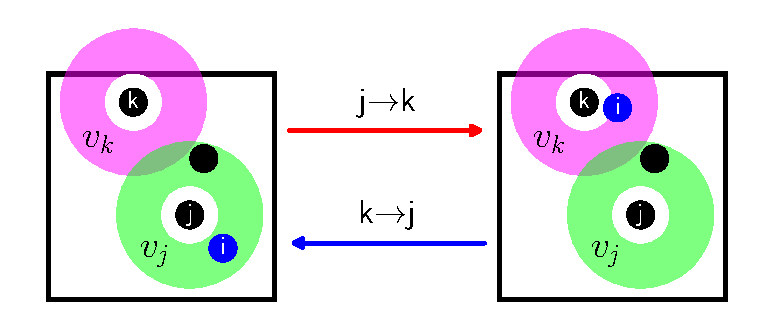
\includegraphics[width=6.5cm]{../figures/avb4.pdf}
\caption{
AVBMC4 displacement of a blue particle of type $m$ from inside the AV, $v_j$ of an existing target particle of type $j$, into the AV of an existing target particle $k$, $v_k$, and the reverse trial.
AVBMC3 does not allow overlapping AV as shown here \cite{chen_improving_2001}.
}
\label{fig:avbmc4}
\end{centering}
\end{figure}

In addition to moves inside and outside of AVs, such as AVBMC2 as described in Section~\ref{sec:lhs_disp_avb2}, moves from one AV to another are also possible, as done in AVBMC3 \cite{chen_improving_2001}.
In this case, two target particles are randomly chosen, and a third mobile particle is moved from the AV of the first target into the AV of the second target.
In the original formulation, AVBMC2 type moves were also considered.
To simplify the acceptance criteria, the AV of the two target particles also could not overlap.
In this section, we describe a variation of AVBMC3, here called AVBMC4 \cite{siderius_flat-histogram_2024}, with two subtle differences from AVBMC3.
First, AVBMC4 does not contain AVBMC2 ``in $\rightarrow$ out" or "out $\rightarrow$ in" moves.
Second, AVBMC4 allows the AV of the target particles to overlap, as long as the two target particles are not inside the AV of the other.

The AVBMC4 trial proceeds as follows.
Two target particles are chosen randomly from all particles of type $j$ and $k$, respectively.
If types $j$ and $k$ are the same, then $\delta_{jk}=1$ and particle $k$ is chosen randomly from $N_k-1$ particles because it cannot be the identical particle $j$.
The AV of the $j$ particle, $v_j$, is defined about one specific site in the $j$ particle.
Similarly, the AV of the $k$ particle, $v_k$, is defined about a specific site in the $k$ particle.
Choose a $k\rightarrow j$ attempt with probability $P_{bias}$, otherwise attempt a $j\rightarrow k$ trial.
For a $j\rightarrow k$ attempt, a mobile particle of type $i$ that has a specific site inside $v_j$, but is not the same particle as the first two chosen $j$ and $k$ particles, is then moved inside $v_k$.
If the $i$ particle has multiple sites or orientation, then it should be randomly oriented or randomly regrown with CB.
For a $k\rightarrow j$ attempt, a mobile particle of type $i$ that has a specific site inside $v_k$, but is not the same particle as the first two chosen $j$ and $k$ particles, is then moved inside $v_j$.

Because $v_j$ and $v_k$ may overlap in AVBMC4, there are a few extra caveats to consider.
If the interaction site in particle $i$ is already inside $v_k$ at the beginning of the trial, then $\Delta_{ik}=1$ and there are $N_i^{in,k} - \Delta_{ik} + 1$ available sites to choose the mobile particle in the reverse move from $v_k$ to $v_j$.
Furthermore, the two targets, $j$ and $k$, cannot be inside the AV of each other, or the trial is rejected.
This trial is summarized in Table~\ref{tab:lhs_disp_avb34}.

\begin{table}
\begin{center}
\begin{tabular}{|c|c|}
 \hline
 \thead{Forward} & \thead{$\alpha_{o\rightarrow n}$} \\ [0.5ex]
 \hline
 Choose $j\rightarrow k$ & $1-P_{bias}$ \\
 \hline
 Choose particle of type $j$ & $1/N_j$ \\
 \hline
 Choose particle of type $k$ & $1/(N_k-\delta_{jk})$ \\
 \hline
 Choose mobile site in $v_j$ & $1/N_i^{in,j}$ \\
 \hline
 Choose $\mathbf{r}_n$ in $v_k$ & $\diff\mathbf{r}/v_k$ \\
 \hline
 Choose orientation & $P_{\omega n}\diff\boldsymbol{\omega}$ \\
 \hline\hline
 \thead{Reverse} & \thead{$\alpha_{n\rightarrow o}$} \\ [0.5ex]
 \hline
 Choose $k\rightarrow j$ & $P_{bias}$ \\
 \hline
 Choose particle of type $j$ & $1/N_j$ \\
 \hline
 Choose particle of type $k$ & $1/(N_k-\delta_{jk})$ \\
 \hline
 Choose mobile site in $v_k$ & $1/(N_i^{in,k} - \Delta_{ik} + 1)$ \\
 \hline
 Choose $\mathbf{r}_o$ in $v_j$ & $\diff\mathbf{r}/v_j$ \\
 \hline
 Choose orientation & $P_{\omega o}\diff\boldsymbol{\omega}$ \\
 \hline
\end{tabular}
\caption{Particle displacement from one AV to another (AVBMC3/4) transition probabilities.}
\label{tab:lhs_disp_avb34}
\end{center}
\end{table}

Using Table~\ref{tab:lhs_disp_avb34} and substituting Eq.~\ref{eq:rhs_nvt} into Eq.~\ref{eq:detailed_balance}, the acceptance probability for the $j\rightarrow k$ attempt as the forward transition is
\begin{equation}
\chi = \frac{P_{bias}}{1-P_{bias}}\left(\frac{v_k P_{\omega o}}{v_j P_{\omega n}}\right)\frac{N_i^{in,j}}{N_i^{in,k} - \Delta_{ik} + 1}e^{-\beta \Delta U}.
\label{eq:avb4jk}
\end{equation}

The acceptance probability for the $k\rightarrow j$ attempt as the forward transition is obtained by perturbing the $j$ and $k$ in Eq.~\ref{eq:avb4jk} and inverting the $P_{bias}$ term to yield
\begin{equation}
\chi = \frac{1-P_{bias}}{P_{bias}}\left(\frac{v_j P_{\omega o}}{v_k P_{\omega n}}\right)\frac{N_i^{in,k}}{N_i^{in,j} - \Delta_{ij} + 1}e^{-\beta \Delta U}.
\label{eq:avb3inin}
\end{equation}


%%%%%%%%%%%%%%%%%%%%%%%%%
\subsection{\label{sec:lhs_disp_cb}Translation with configurational bias (CB)}
%%%%%%%%%%%%%%%%%%%%%%%%%

While configurational bias (CB) is often used to grow complex molecules, CB may also be used to translate particles.
Although this may not be the most efficient choice for many applications, it is instructive to consider how CB is derived.
In addition, dual-cut configurational (DCCB) \cite{vlugt_improving_1998} may make this an efficient trial.
To our knowledge, CB on single site translation has not been published before.

A CB translation proceeds as follows.
A particle is randomly chosen among all mobile, non-fixed particles in the old microstate, $N_m=\sum_i^{mobile} N_i$, where $i$ is the particle type.
%A particle of type $i$ is chosen randomly.
The position of a specific site in the chosen particle is $\mathbf{r}_o$ at the beginning of the trial.
Then, $c$ new positions, $\mathbf{r}_n^i$, are placed at random positions selected uniformly within $\pm\delta/2$ of $\mathbf{r}_o$ in each of $D$ dimensions.
One of the $c$ positions are chosen with probability $\pi_{cn}$, and the particle is rigidly translated to that position with fixed orientation.
The $\pi_{cn}$ may be a function of the positions of the particles, and this choice is the namesake of the CB method \cite{siepmann_configurational_1992}.
The reverse trial is to choose the same particle of type $i$, and translated from $\mathbf{r}_n$ to $\mathbf{r}_o$ after choosing from among $c$ positions with probability $\pi_{co}$.
The probability $\pi_{co}$ is used in choosing a new position about $\mathbf{r}_n$, while $\pi_{cn}$ is used in choosing a new position about $\mathbf{r}_o$.
Fig.~\ref{fig:dccb_draw} shows an illustrative example of $\pi_{co} \neq \pi_{cn}$.

\begin{figure}
\begin{centering}
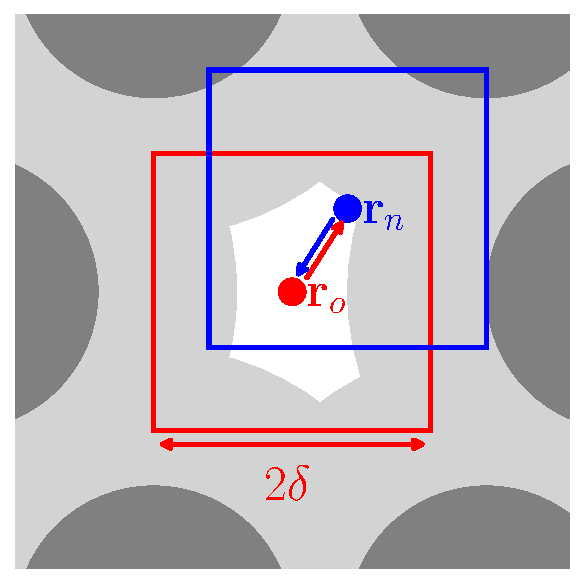
\includegraphics[width=4.5cm]{../figures/dccb_draw.pdf}
\caption{
An illustration of the old and new Rosenbluth terms for hard circles as described in Fig.~\ref{fig:lhs_nvt}.
The red box shows the positions available to $\pi_{cn}$ while the blue box shows the positions available to $\pi_{co}$.
Although the entire free volume is available to $\pi_{cn}$, it is not all available to $\pi_{co}$.
Thus, $\pi_{cn} \neq \pi_{co}$.
}
\label{fig:dccb_draw}
\end{centering}
\end{figure}

\begin{table}
\begin{center}
\begin{tabular}{|c|c|}
 \hline
 \thead{Forward} & \thead{$\alpha_{o\rightarrow n}$} \\ [0.5ex]
 \hline
 Choose from $N_m$ & $1/N_m$ \\
 \hline
 \makecell{Choose $c$ positions about $\mathbf{r}_o$.\\ Probability that $\mathbf{r}_n$ is in $c$.} & $c\diff\mathbf{r}/\delta^D$ \\
 \hline
 Choose $\mathbf{r}_n$ in $c$ positions & $\pi_{cn}$ \\
 \hline\hline
 \thead{Reverse} & \thead{$\alpha_{n\rightarrow o}$} \\ [0.5ex]
 \hline
 Choose from $N_m$ & $1/N_m$ \\
 \hline
 \makecell{Choose $c$ positions about $\mathbf{r}_n$.\\ Probability that $\mathbf{r}_o$ is in $c$.} & $c\diff\mathbf{r}/\delta^D$ \\
 \hline
 Choose $\mathbf{r}_o$ in $c$ positions & $\pi_{co}$ \\
 \hline
\end{tabular}
\caption{Translation with CB transition probabilities.}
\label{tab:lhs_disp_cb}
\end{center}
\end{table}

The transition probabilities are summarized in Table~\ref{tab:lhs_disp_cb}.
Using Table~\ref{tab:lhs_disp_cb} and substituting Eq.~\ref{eq:rhs_nvt} into Eq.~\ref{eq:detailed_balance}, the acceptance probability is
\begin{equation}
\chi = \frac{\pi_{co}}{\pi_{cn}}e^{-\beta \Delta U}.
\label{eq:cb}
\end{equation}

There is remarkable flexibility in the choice of $c$ positions, $\pi_{cn}$.
An often-used functional form is given by
\begin{equation}
\pi_{cn}=\frac{e^{-\beta U(\mathbf{r}_n)}}{W_{cn}},
\label{eq:pcn}
\end{equation}
where $W_{cn}=\sum_{in}^c e^{-\beta U(\mathbf{r}_{in})}$ and the subscript $in$ denotes that the positions, $\mathbf{r}_{in}$, were placed at random positions selected uniformly about $\mathbf{r}_o$ and contain $\mathbf{r}_n$.
Similarly, $\pi_{co}$ is given by
\begin{equation}
\pi_{co}=\frac{e^{-\beta U(\mathbf{r}_o)}}{W_{co}}
\label{eq:pco}
\end{equation}
where $W_{co}=\sum_{io}^c e^{-\beta U(\mathbf{r}_{io})}$ and the subscript $io$ denotes that the positions, $\mathbf{r}_{io}$, were placed at random positions selected uniformly about $\mathbf{r}_n$ and contain $\mathbf{r}_o$.

Substituting Eqs.~\ref{eq:pcn} and \ref{eq:pco} into Eq.~\ref{eq:cb} gives
\begin{equation}
\chi = \frac{W_{cn}}{W_{co}}e^{-\beta[\Delta U - U(\mathbf{r}_n) + U(\mathbf{r}_o)]}.
\end{equation}
This form of $\pi_{cn}$ is convenient because $\Delta U - U(\mathbf{r}_n) + U(\mathbf{r}_o)$ contains only interaction energies beyond the center of the first site (e.g., if there were multiple sites).

The efficiency of translation CB is debatable and depends upon the model system.
Standard translations for single-site isotropic particles described in Section~\ref{sec:lhs_translation} may be more optimal for the following reason.
Assuming that the calculation of the energy takes the majority of the CPU time, a standard translation requires computing the energy twice (or only once if the old contribution is stored).
In comparison, this choice of $\pi_{cn}$ and $\pi_{co}$ requires computing the energy $2c$ times (minus one if the old contribution is stored).
Thus, in the CPU time it takes to complete one of these CB trials, approximately $c$ standard trials could have been attempted, each with their own acceptance probability.
In this case, its possible more than one of the $c$ standard trials could have been accepted, in which case the standard approach would be more efficient.

On the other hand, other choices of $\pi_{cn}$ and $\pi_{co}$ could make CB translation efficient, even for single-site particles, as we will show in the next section.

%%%%%%%%%%%%%%%%%%%%%%%%%
\subsection{\label{sec:lhs_disp_dccb}Translation with dual-cut configurational bias (DCCB)}
%%%%%%%%%%%%%%%%%%%%%%%%%

A more efficient choice of $\pi_{cn}$ and $\pi_{co}$ is the DCCB approach if a suitable reference potential may be utilized \cite{vlugt_improving_1998}.
The namesake of DCCB is to apply a shorter cutoff to the energy calculation in $\pi_{cn}$ and $\pi_{co}$, but here we generalize dual-cut to include any reference potential, $U_r$, that takes less CPU time than the full potential, as discussed in Section~\ref{sec:lhs_insdel_cb}.
For DCCB,
\begin{equation}
\pi_{cn}=\frac{e^{-\beta U_r(\mathbf{r}_n)}}{W_{cnr}},
\label{eq:pcnr}
\end{equation}
where $W_{cnr}=\sum_{in}^c e^{-\beta U_r(\mathbf{r}_{in})}$ and the subscript $in$ denotes that the positions, $\mathbf{r}_{in}$, were placed at random positions selected uniformly about $\mathbf{r}_o$.
The acceptance criteria is then obtained by substituting Eq.~\ref{eq:pcnr} for both $\pi_{cn}$ and $\pi_{co}$ in Eq.~\ref{eq:cb},
\begin{equation}
\chi = \frac{W_{cnr}}{W_{cor}}e^{-\beta [\Delta U - U_r(\mathbf{r}_n) + U_r(\mathbf{r}_o)]}.
\end{equation}
Assuming that $U_r$ results in the choice of likely accepted configurations by approximating the highest-contributing parts of the full potential, the sampling efficiency may be increased.
On the other hand, a poor choice of $U_r$ could decrease the simulation efficiency.
In the worst case, ergodic sampling is broken by the rejection of valid configurations due to a poor reference potential, and the simulation results could be wrong.
Despite this, DCCB is an efficient method that may be tested and benchmarked against simulations without DCCB.

%%%%%%%%%%%%%%%%%%%%%%%%%
\subsection{\label{sec:lhs_cluster}Translation and rotation of rigid clusters}
%%%%%%%%%%%%%%%%%%%%%%%%%

The translation of rigid clusters is very similar to that of single particles described in Section~\ref{sec:lhs_translation}, except for the key differences that a cluster criteria must be specified, and that particles identified as part of a cluster must stay in that cluster after the trial.
If the clusters are allowed to change, then detailed balance is violated, as shown in Fig.~\ref{fig:cluster}.
Rigid cluster trial moves are biased because the transition probabilities depend on the configuration (i.e., the cluster criteria).

\begin{figure}
\begin{centering}
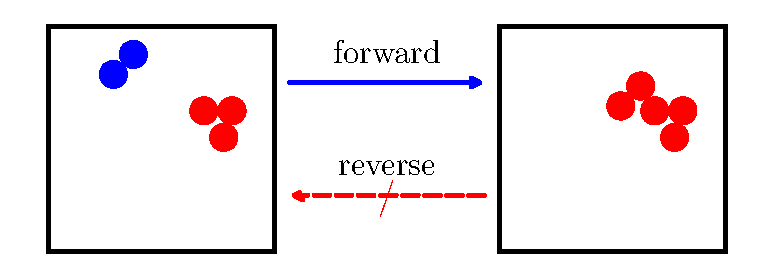
\includegraphics[width=6.5cm]{../figures/cluster.pdf}
\caption{
Detailed balance is violated if two separate clusters coalesce during a rigid cluster translation.
In the forward transition, the blue cluster is translated near a separate cluster shown in red.
If this move were allowed, the reverse cluster move would be impossible because clusters are moved rigidly and cannot be broken apart during the trial.
To obey detailed balance, reject rigid cluster moves that result in the coalescence of two originally separate clusters.
}
\label{fig:cluster}
\end{centering}
\end{figure}

A rigid cluster translation or rotation proceeds as follows.
First, an individual cluster is identified.
This identification could take many forms.
For example, one particle could be randomly chosen for a given type, and then a flood-fill algorithm could be used to find all particles within a distance cutoff from all particles in the cluster \cite{hatch_self-assembly_2016}.
Regardless of the metric used to identify clusters, the same metric must be applied again at the end of the trial.
In addition, if a cluster has picked up or lost any particles, then the trial must be immediately rejected.
Clusters may be rigidly translated or rotated with a parameter that is tunable during equilibration but must stay constant during production simulations, as described in Section~\ref{sec:lhs_translation}.
The acceptance criteria is then given by Eq.~\ref{eq:lhs_translate} or \ref{eq:lhs_rotate}.
